\documentclass[]{article}
\usepackage{lmodern}
\usepackage{amssymb,amsmath}
\usepackage{ifxetex,ifluatex}
\usepackage{fixltx2e} % provides \textsubscript
\ifnum 0\ifxetex 1\fi\ifluatex 1\fi=0 % if pdftex
  \usepackage[T1]{fontenc}
  \usepackage[utf8]{inputenc}
\else % if luatex or xelatex
  \ifxetex
    \usepackage{mathspec}
  \else
    \usepackage{fontspec}
  \fi
  \defaultfontfeatures{Ligatures=TeX,Scale=MatchLowercase}
\fi
% use upquote if available, for straight quotes in verbatim environments
\IfFileExists{upquote.sty}{\usepackage{upquote}}{}
% use microtype if available
\IfFileExists{microtype.sty}{%
\usepackage{microtype}
\UseMicrotypeSet[protrusion]{basicmath} % disable protrusion for tt fonts
}{}
\usepackage[margin=1in]{geometry}
\usepackage{hyperref}
\PassOptionsToPackage{usenames,dvipsnames}{color} % color is loaded by hyperref
\hypersetup{unicode=true,
            pdftitle={Lab 02},
            colorlinks=true,
            linkcolor=Maroon,
            citecolor=Blue,
            urlcolor=Blue,
            breaklinks=true}
\urlstyle{same}  % don't use monospace font for urls
\usepackage{color}
\usepackage{fancyvrb}
\newcommand{\VerbBar}{|}
\newcommand{\VERB}{\Verb[commandchars=\\\{\}]}
\DefineVerbatimEnvironment{Highlighting}{Verbatim}{commandchars=\\\{\}}
% Add ',fontsize=\small' for more characters per line
\usepackage{framed}
\definecolor{shadecolor}{RGB}{248,248,248}
\newenvironment{Shaded}{\begin{snugshade}}{\end{snugshade}}
\newcommand{\AlertTok}[1]{\textcolor[rgb]{0.94,0.16,0.16}{#1}}
\newcommand{\AnnotationTok}[1]{\textcolor[rgb]{0.56,0.35,0.01}{\textbf{\textit{#1}}}}
\newcommand{\AttributeTok}[1]{\textcolor[rgb]{0.77,0.63,0.00}{#1}}
\newcommand{\BaseNTok}[1]{\textcolor[rgb]{0.00,0.00,0.81}{#1}}
\newcommand{\BuiltInTok}[1]{#1}
\newcommand{\CharTok}[1]{\textcolor[rgb]{0.31,0.60,0.02}{#1}}
\newcommand{\CommentTok}[1]{\textcolor[rgb]{0.56,0.35,0.01}{\textit{#1}}}
\newcommand{\CommentVarTok}[1]{\textcolor[rgb]{0.56,0.35,0.01}{\textbf{\textit{#1}}}}
\newcommand{\ConstantTok}[1]{\textcolor[rgb]{0.00,0.00,0.00}{#1}}
\newcommand{\ControlFlowTok}[1]{\textcolor[rgb]{0.13,0.29,0.53}{\textbf{#1}}}
\newcommand{\DataTypeTok}[1]{\textcolor[rgb]{0.13,0.29,0.53}{#1}}
\newcommand{\DecValTok}[1]{\textcolor[rgb]{0.00,0.00,0.81}{#1}}
\newcommand{\DocumentationTok}[1]{\textcolor[rgb]{0.56,0.35,0.01}{\textbf{\textit{#1}}}}
\newcommand{\ErrorTok}[1]{\textcolor[rgb]{0.64,0.00,0.00}{\textbf{#1}}}
\newcommand{\ExtensionTok}[1]{#1}
\newcommand{\FloatTok}[1]{\textcolor[rgb]{0.00,0.00,0.81}{#1}}
\newcommand{\FunctionTok}[1]{\textcolor[rgb]{0.00,0.00,0.00}{#1}}
\newcommand{\ImportTok}[1]{#1}
\newcommand{\InformationTok}[1]{\textcolor[rgb]{0.56,0.35,0.01}{\textbf{\textit{#1}}}}
\newcommand{\KeywordTok}[1]{\textcolor[rgb]{0.13,0.29,0.53}{\textbf{#1}}}
\newcommand{\NormalTok}[1]{#1}
\newcommand{\OperatorTok}[1]{\textcolor[rgb]{0.81,0.36,0.00}{\textbf{#1}}}
\newcommand{\OtherTok}[1]{\textcolor[rgb]{0.56,0.35,0.01}{#1}}
\newcommand{\PreprocessorTok}[1]{\textcolor[rgb]{0.56,0.35,0.01}{\textit{#1}}}
\newcommand{\RegionMarkerTok}[1]{#1}
\newcommand{\SpecialCharTok}[1]{\textcolor[rgb]{0.00,0.00,0.00}{#1}}
\newcommand{\SpecialStringTok}[1]{\textcolor[rgb]{0.31,0.60,0.02}{#1}}
\newcommand{\StringTok}[1]{\textcolor[rgb]{0.31,0.60,0.02}{#1}}
\newcommand{\VariableTok}[1]{\textcolor[rgb]{0.00,0.00,0.00}{#1}}
\newcommand{\VerbatimStringTok}[1]{\textcolor[rgb]{0.31,0.60,0.02}{#1}}
\newcommand{\WarningTok}[1]{\textcolor[rgb]{0.56,0.35,0.01}{\textbf{\textit{#1}}}}
\usepackage{graphicx,grffile}
\makeatletter
\def\maxwidth{\ifdim\Gin@nat@width>\linewidth\linewidth\else\Gin@nat@width\fi}
\def\maxheight{\ifdim\Gin@nat@height>\textheight\textheight\else\Gin@nat@height\fi}
\makeatother
% Scale images if necessary, so that they will not overflow the page
% margins by default, and it is still possible to overwrite the defaults
% using explicit options in \includegraphics[width, height, ...]{}
\setkeys{Gin}{width=\maxwidth,height=\maxheight,keepaspectratio}
\IfFileExists{parskip.sty}{%
\usepackage{parskip}
}{% else
\setlength{\parindent}{0pt}
\setlength{\parskip}{6pt plus 2pt minus 1pt}
}
\setlength{\emergencystretch}{3em}  % prevent overfull lines
\providecommand{\tightlist}{%
  \setlength{\itemsep}{0pt}\setlength{\parskip}{0pt}}
\setcounter{secnumdepth}{0}
% Redefines (sub)paragraphs to behave more like sections
\ifx\paragraph\undefined\else
\let\oldparagraph\paragraph
\renewcommand{\paragraph}[1]{\oldparagraph{#1}\mbox{}}
\fi
\ifx\subparagraph\undefined\else
\let\oldsubparagraph\subparagraph
\renewcommand{\subparagraph}[1]{\oldsubparagraph{#1}\mbox{}}
\fi

%%% Use protect on footnotes to avoid problems with footnotes in titles
\let\rmarkdownfootnote\footnote%
\def\footnote{\protect\rmarkdownfootnote}


  \title{Lab 02}
    \author{}
    \date{}
  

% change section title styling
\usepackage{sectsty}
\sectionfont{\normalsize\normalfont\itshape}
\subsectionfont{\normalsize\normalfont}

% use fancyhdr style
\usepackage{fancyhdr}
\pagestyle{fancy}
\fancyhead[LO, LE]{Lab 02}
\fancyhead[RO, RE]{GEOG 491/891}
\makeatletter
\renewcommand{\maketitle}{\bgroup\vspace*{-1cm}\setlength{\parindent}{0pt}
\begin{flushleft}
  \@author
  
  \@date
  
\end{flushleft}\egroup
}
\makeatother

\begin{document}
\maketitle

\hypertarget{lab-02-r-as-a-gis}{%
\section{Lab 02: R as a GIS}\label{lab-02-r-as-a-gis}}

\hypertarget{read-the-instructions-completely-before-starting-the-lab}{%
\subsubsection{Read the instructions COMPLETELY before starting the
lab}\label{read-the-instructions-completely-before-starting-the-lab}}

This lab builds on many of the discussions and exercises from class,
including previous labs.

\hypertarget{formatting-your-submission}{%
\subsubsection{Formatting your
submission}\label{formatting-your-submission}}

This lab must be placed into a public repository on GitHub
(www.github.com). Before the due date, submit \textbf{on Canvas} a link
to the repository. I will then download your repositories and run your
code. The code must be contained in either a .R script or a .Rmd
markdown document. As I need to run your code, any data you use in the
lab must be referenced using \textbf{relative path names}. Finally,
answers to questions I pose in this document must also be in the
repository at the time you submit your link to Canvas. They can be in a
separate text file, or if you decide to use an RMarkdown document, you
can answer them directly in the doc.

\hypertarget{data}{%
\subsection{Data}\label{data}}

The data for this lab can be found in the \texttt{./data/CBW/} directory
within the course GitHub repository.

Spatial datasets:

\begin{enumerate}
\def\labelenumi{\arabic{enumi}.}
\item
  Streams\_Opened\_by\_Dam\_Removal\_2012\_2017.shp
\item
  Dam\_or\_Other\_Blockage\_Removed\_2012\_2017.shp
\item
  County\_Boundaries.shp
\end{enumerate}

Non-spatial datasets

\begin{enumerate}
\def\labelenumi{\arabic{enumi}.}
\tightlist
\item
  BMPreport2016\_landbmps.csv
\end{enumerate}

\hypertarget{working-with-tabular-data}{%
\subsection{Working with tabular data}\label{working-with-tabular-data}}

\begin{Shaded}
\begin{Highlighting}[]
\CommentTok{\# setup}
\FunctionTok{library}\NormalTok{(tidyverse)}
\end{Highlighting}
\end{Shaded}

\begin{verbatim}
## -- Attaching packages --------------------------------------- tidyverse 1.3.1 --
\end{verbatim}

\begin{verbatim}
## v ggplot2 3.3.5     v purrr   0.3.4
## v tibble  3.1.2     v dplyr   1.0.7
## v tidyr   1.1.3     v stringr 1.4.0
## v readr   1.4.0     v forcats 0.5.1
\end{verbatim}

\begin{verbatim}
## -- Conflicts ------------------------------------------ tidyverse_conflicts() --
## x dplyr::filter() masks stats::filter()
## x dplyr::lag()    masks stats::lag()
\end{verbatim}

\begin{Shaded}
\begin{Highlighting}[]
\FunctionTok{library}\NormalTok{(sf)}
\end{Highlighting}
\end{Shaded}

\begin{verbatim}
## Linking to GEOS 3.8.1, GDAL 3.2.1, PROJ 7.2.1
\end{verbatim}

\begin{Shaded}
\begin{Highlighting}[]
\FunctionTok{library}\NormalTok{(tmap)}
\end{Highlighting}
\end{Shaded}

A ``join'' is a method to join multiple tables together using a matching
``key'' found in both datasets. For example:

\begin{Shaded}
\begin{Highlighting}[]
\CommentTok{\# table of names}
\NormalTok{t.names }\OtherTok{\textless{}{-}} \FunctionTok{tibble}\NormalTok{(}\AttributeTok{key =} \FunctionTok{c}\NormalTok{(}\DecValTok{1}\NormalTok{, }\DecValTok{2}\NormalTok{, }\DecValTok{3}\NormalTok{), }
             \AttributeTok{name =} \FunctionTok{c}\NormalTok{(}\StringTok{"Huey"}\NormalTok{, }\StringTok{"Dewey"}\NormalTok{, }\StringTok{"Louis"}\NormalTok{))}

\CommentTok{\# table of scores}
\NormalTok{t.scores }\OtherTok{\textless{}{-}} \FunctionTok{tibble}\NormalTok{(}\AttributeTok{name =} \FunctionTok{c}\NormalTok{(}\StringTok{"Louis"}\NormalTok{, }\StringTok{"Huey"}\NormalTok{, }\StringTok{"Dewey"}\NormalTok{),}
                   \AttributeTok{grade =} \FunctionTok{c}\NormalTok{(}\DecValTok{99}\NormalTok{, }\DecValTok{45}\NormalTok{, }\DecValTok{33}\NormalTok{))}

\CommentTok{\# combined them}
\NormalTok{t.joined }\OtherTok{\textless{}{-}} \FunctionTok{left\_join}\NormalTok{(t.names, t.scores, }\AttributeTok{by =} \StringTok{"name"}\NormalTok{)}
\NormalTok{t.joined}
\end{Highlighting}
\end{Shaded}

\begin{verbatim}
## # A tibble: 3 x 3
##     key name  grade
##   <dbl> <chr> <dbl>
## 1     1 Huey     45
## 2     2 Dewey    33
## 3     3 Louis    99
\end{verbatim}

A ``left join'' finds starts with the table on the ``left'' and then
finds matches in the table on the ``right''. See the documentation using
\texttt{?left\_join} for more details and for other types of joins.
Sometimes the attributes you're using to join the tables won't have the
same name, in which case the syntax is different:

\begin{Shaded}
\begin{Highlighting}[]
\NormalTok{t.wonkyNames }\OtherTok{\textless{}{-}} \FunctionTok{tibble}\NormalTok{(}\AttributeTok{nombre =} \FunctionTok{c}\NormalTok{(}\StringTok{"Dewey"}\NormalTok{, }\StringTok{"Louis"}\NormalTok{, }\StringTok{"Huey"}\NormalTok{),}
                       \AttributeTok{x =} \FunctionTok{rep}\NormalTok{(}\DecValTok{999}\NormalTok{),}
                       \AttributeTok{favoriteFood =} \FunctionTok{c}\NormalTok{(}\StringTok{"banana"}\NormalTok{, }\StringTok{"apple"}\NormalTok{, }\StringTok{"carrot"}\NormalTok{))}

\NormalTok{t.joined2 }\OtherTok{\textless{}{-}} \FunctionTok{left\_join}\NormalTok{(t.names, t.wonkyNames, }\AttributeTok{by =} \FunctionTok{c}\NormalTok{(}\StringTok{"name"} \OtherTok{=} \StringTok{"nombre"}\NormalTok{))}
\NormalTok{t.joined2}
\end{Highlighting}
\end{Shaded}

\begin{verbatim}
## # A tibble: 3 x 4
##     key name      x favoriteFood
##   <dbl> <chr> <dbl> <chr>       
## 1     1 Huey    999 carrot      
## 2     2 Dewey   999 banana      
## 3     3 Louis   999 apple
\end{verbatim}

\hypertarget{lets-take-a-look-at-some-tabular-data}{%
\subsection{Let's take a look at some tabular
data}\label{lets-take-a-look-at-some-tabular-data}}

This dataset includes a list of best management practices (``BMPs'') to
reduce nutrient and sediment pollution in the Chesapeake Bay Watershed.

\begin{Shaded}
\begin{Highlighting}[]
\NormalTok{bmps }\OtherTok{\textless{}{-}} \FunctionTok{read\_csv}\NormalTok{(}\StringTok{"../data/CBW/BMPreport2016\_landbmps.csv"}\NormalTok{)}
\end{Highlighting}
\end{Shaded}

\begin{verbatim}
## 
## -- Column specification --------------------------------------------------------
## cols(
##   StateAbbreviation = col_character(),
##   GeographyName = col_character(),
##   Geography = col_character(),
##   Agency = col_character(),
##   BMPShortName = col_character(),
##   BMP = col_character(),
##   BMPType = col_character(),
##   Unit = col_character(),
##   Sector = col_character(),
##   FromLoadSource = col_character(),
##   ToLoadSource = col_character(),
##   AmountSubmitted = col_double(),
##   AmountBackedOut = col_double(),
##   AmountNotBackedOut = col_double(),
##   AmountCredited = col_double(),
##   Excess = col_double(),
##   TotalAmountCredited = col_double(),
##   Cost = col_double()
## )
\end{verbatim}

\begin{Shaded}
\begin{Highlighting}[]
\FunctionTok{glimpse}\NormalTok{(bmps)}
\end{Highlighting}
\end{Shaded}

\begin{verbatim}
## Rows: 69,601
## Columns: 18
## $ StateAbbreviation   <chr> "DC", "DC", "DC", "DC", "DC", "DC", "DC", "DC", "D~
## $ GeographyName       <chr> "11001(cbwsonly)", "11001(cbwsonly)", "11001(cbwso~
## $ Geography           <chr> "Washington, DC (CBWS Portion Only)", "Washington,~
## $ Agency              <chr> "Department of Defense", "Department of Defense", ~
## $ BMPShortName        <chr> "wetpondwetland", "wetpondwetland", "wetpondwetlan~
## $ BMP                 <chr> "Wet Ponds and Wetlands", "Wet Ponds and Wetlands"~
## $ BMPType             <chr> "Efficiency", "Efficiency", "Efficiency", "Efficie~
## $ Unit                <chr> "Acres Treated", "Acres Treated", "Acres Treated",~
## $ Sector              <chr> "Developed", "Developed", "Developed", "Developed"~
## $ FromLoadSource      <chr> "Non-Regulated Roads", "Non-Regulated Buildings an~
## $ ToLoadSource        <chr> "Non-Regulated Roads", "Non-Regulated Buildings an~
## $ AmountSubmitted     <dbl> 8.709123261, 47.984171150, 1.358309392, 6.76626660~
## $ AmountBackedOut     <dbl> 0, 0, 0, 0, 0, 0, 0, 0, 0, 0, 0, 0, 0, 0, 0, 0, 0,~
## $ AmountNotBackedOut  <dbl> 8.709123261, 47.984171150, 1.358309392, 6.76626660~
## $ AmountCredited      <dbl> 8.709123261, 47.984171150, 1.358309392, 6.76626660~
## $ Excess              <dbl> 0, 0, 0, 0, 0, 0, 0, 0, 0, 0, 0, 0, 0, 0, 0, 0, 0,~
## $ TotalAmountCredited <dbl> 8.709123261, 47.984171150, 1.358309392, 6.76626660~
## $ Cost                <dbl> 11462.077120, 63151.967650, 1787.670991, 8905.0834~
\end{verbatim}

Look at the attribute ``GeographyName'' - it's a character attribute
that contains the counties' FIPS code, but also some ancillary
explanatory data we need to get rid of. There are multiple ways of doing
so, including some (very) fancy automated methods that detect patterns
of numbers and characters. We're going to take a simpler approach and
assume that all FIPS codes are only 5 characters long.

\begin{Shaded}
\begin{Highlighting}[]
\CommentTok{\# edit the bmps variable in place, which isn\textquotesingle{}t always best practices}
\NormalTok{bmps }\OtherTok{\textless{}{-}}\NormalTok{ bmps }\SpecialCharTok{\%\textgreater{}\%} \FunctionTok{mutate}\NormalTok{(., }\AttributeTok{FIPS.trimmed =}\NormalTok{ stringr}\SpecialCharTok{::}\FunctionTok{str\_sub}\NormalTok{(GeographyName, }\DecValTok{1}\NormalTok{, }\DecValTok{5}\NormalTok{))}
\end{Highlighting}
\end{Shaded}

This can be sueful when you're trying to create ``keys'' by which to
join tables or just clean your tables in general

Let's recall how to do some simple tasks

\begin{Shaded}
\begin{Highlighting}[]
\CommentTok{\# Let\textquotesingle{}s calculate the total cost by BMP and then plot it}
\NormalTok{bmps }\SpecialCharTok{\%\textgreater{}\%} \FunctionTok{group\_by}\NormalTok{(BMPType) }\SpecialCharTok{\%\textgreater{}\%} \FunctionTok{summarise}\NormalTok{(}\AttributeTok{totalCost =} \FunctionTok{sum}\NormalTok{(Cost)) }\SpecialCharTok{\%\textgreater{}\%}
  \FunctionTok{ggplot}\NormalTok{(., }\FunctionTok{aes}\NormalTok{(}\AttributeTok{x =}\NormalTok{ BMPType, }\AttributeTok{y =}\NormalTok{ totalCost)) }\SpecialCharTok{+}
  \FunctionTok{geom\_bar}\NormalTok{(}\AttributeTok{stat =} \StringTok{"identity"}\NormalTok{) }\SpecialCharTok{+}
  \FunctionTok{theme\_minimal}\NormalTok{()}
\end{Highlighting}
\end{Shaded}

\begin{verbatim}
## Warning: Removed 2 rows containing missing values (position_stack).
\end{verbatim}

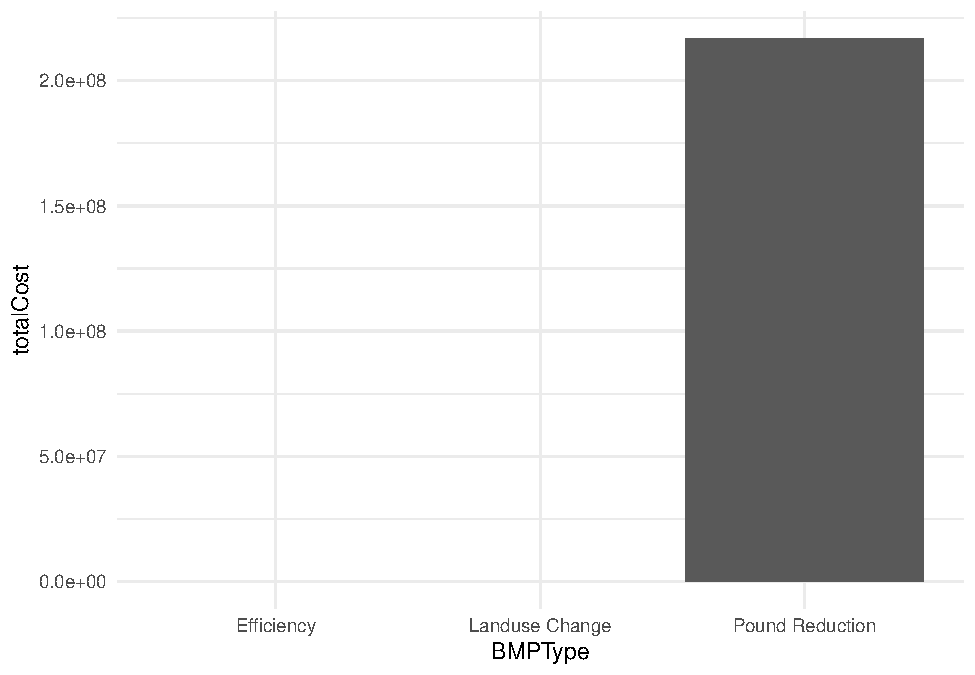
\includegraphics{lab02_files/figure-latex/review-1.pdf}

\begin{Shaded}
\begin{Highlighting}[]
\CommentTok{\# Doesn\textquotesingle{}t really work. This is because there are missing data in the cost attribute. Let\textquotesingle{}s look at it (and this is why we do exploratory data analysis first)}

\FunctionTok{summary}\NormalTok{(bmps}\SpecialCharTok{$}\NormalTok{Cost)}
\end{Highlighting}
\end{Shaded}

\begin{verbatim}
##     Min.  1st Qu.   Median     Mean  3rd Qu.     Max.     NA's 
##        0        0      142    37408     3583 39731974    14286
\end{verbatim}

\begin{Shaded}
\begin{Highlighting}[]
\CommentTok{\# Yup, lots of "NA\textquotesingle{}s"... We can drop them in our analysis. Look carefully at the code in the \textquotesingle{}sum\textquotesingle{} function}


\NormalTok{bmps }\SpecialCharTok{\%\textgreater{}\%} \FunctionTok{group\_by}\NormalTok{(BMPType) }\SpecialCharTok{\%\textgreater{}\%} \FunctionTok{summarise}\NormalTok{(}\AttributeTok{totalCost =} \FunctionTok{sum}\NormalTok{(Cost, }\AttributeTok{na.rm =}\NormalTok{ T)) }\SpecialCharTok{\%\textgreater{}\%}
  \FunctionTok{ggplot}\NormalTok{(., }\FunctionTok{aes}\NormalTok{(}\AttributeTok{x =}\NormalTok{ BMPType, }\AttributeTok{y =}\NormalTok{ totalCost)) }\SpecialCharTok{+}
  \FunctionTok{geom\_bar}\NormalTok{(}\AttributeTok{stat =} \StringTok{"identity"}\NormalTok{) }\SpecialCharTok{+}
  \FunctionTok{theme\_minimal}\NormalTok{()}
\end{Highlighting}
\end{Shaded}

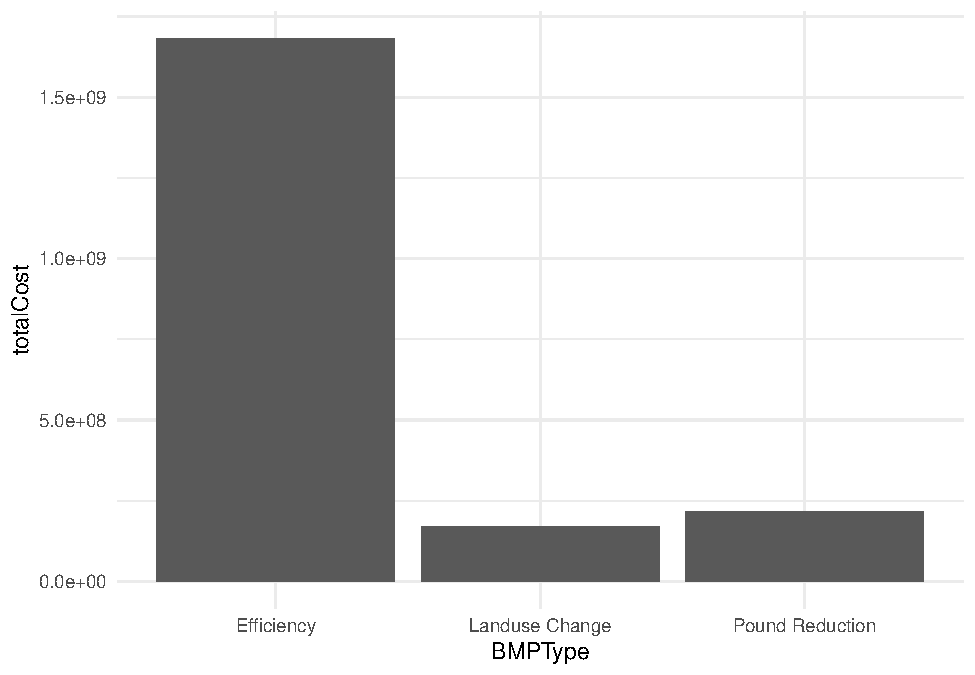
\includegraphics{lab02_files/figure-latex/review-2.pdf}

We can also group by multiple variables at the same time. For example:

\begin{Shaded}
\begin{Highlighting}[]
\CommentTok{\# group by state and sector, sum total cost}
\NormalTok{twofactors }\OtherTok{\textless{}{-}}\NormalTok{ bmps }\SpecialCharTok{\%\textgreater{}\%} \FunctionTok{group\_by}\NormalTok{(StateAbbreviation, Sector) }\SpecialCharTok{\%\textgreater{}\%} \FunctionTok{summarise}\NormalTok{(}\AttributeTok{totalCost =} \FunctionTok{sum}\NormalTok{(Cost))}
\end{Highlighting}
\end{Shaded}

\begin{verbatim}
## `summarise()` has grouped output by 'StateAbbreviation'. You can override using the `.groups` argument.
\end{verbatim}

For our last bit of review, let's make a few box plots:

\begin{Shaded}
\begin{Highlighting}[]
\CommentTok{\# A simple one}
\NormalTok{bmps }\SpecialCharTok{\%\textgreater{}\%} \FunctionTok{ggplot}\NormalTok{(., }\FunctionTok{aes}\NormalTok{(}\AttributeTok{x =}\NormalTok{ StateAbbreviation, }\AttributeTok{y =}\NormalTok{ AmountCredited)) }\SpecialCharTok{+}
  \FunctionTok{geom\_boxplot}\NormalTok{(}\FunctionTok{aes}\NormalTok{(}\AttributeTok{fill =}\NormalTok{ StateAbbreviation))}
\end{Highlighting}
\end{Shaded}

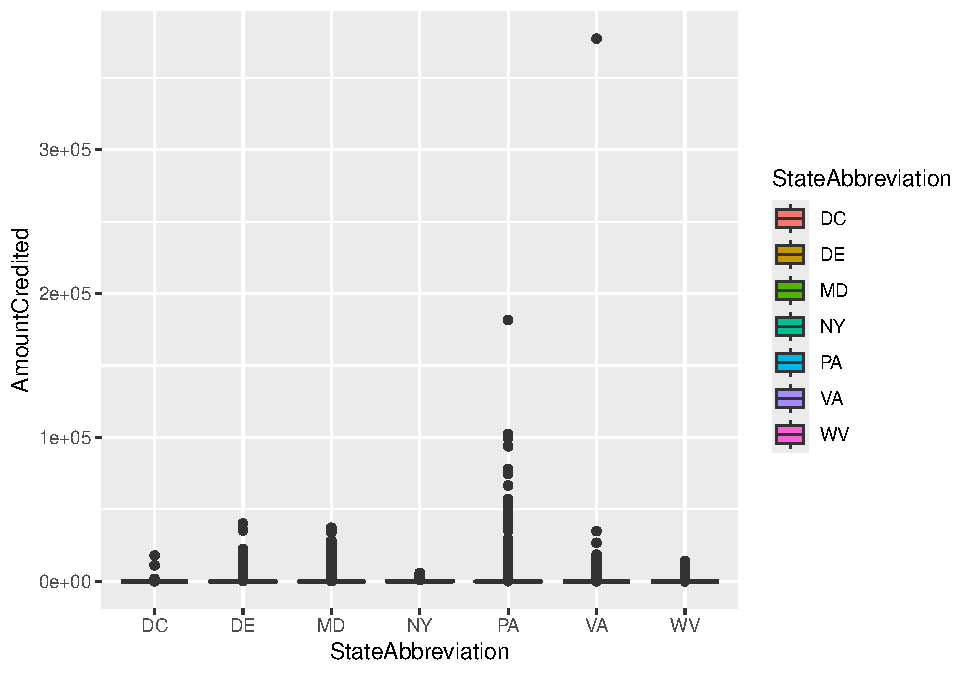
\includegraphics{lab02_files/figure-latex/review3-1.pdf}

\begin{Shaded}
\begin{Highlighting}[]
\CommentTok{\# Very heavily skewed, so just for the sake of visualization, let\textquotesingle{}s subset the data (dramatically)}
\NormalTok{bmps }\SpecialCharTok{\%\textgreater{}\%} 
\NormalTok{  dplyr}\SpecialCharTok{::}\FunctionTok{filter}\NormalTok{(., AmountCredited }\SpecialCharTok{\textgreater{}} \DecValTok{1} \SpecialCharTok{\&}\NormalTok{ AmountCredited }\SpecialCharTok{\textless{}} \DecValTok{100}\NormalTok{) }\SpecialCharTok{\%\textgreater{}\%} 
  \FunctionTok{ggplot}\NormalTok{(., }\FunctionTok{aes}\NormalTok{(}\AttributeTok{x =}\NormalTok{ StateAbbreviation, }\AttributeTok{y =}\NormalTok{ AmountCredited)) }\SpecialCharTok{+}
  \FunctionTok{geom\_boxplot}\NormalTok{(}\FunctionTok{aes}\NormalTok{(}\AttributeTok{fill =}\NormalTok{ StateAbbreviation))}
\end{Highlighting}
\end{Shaded}

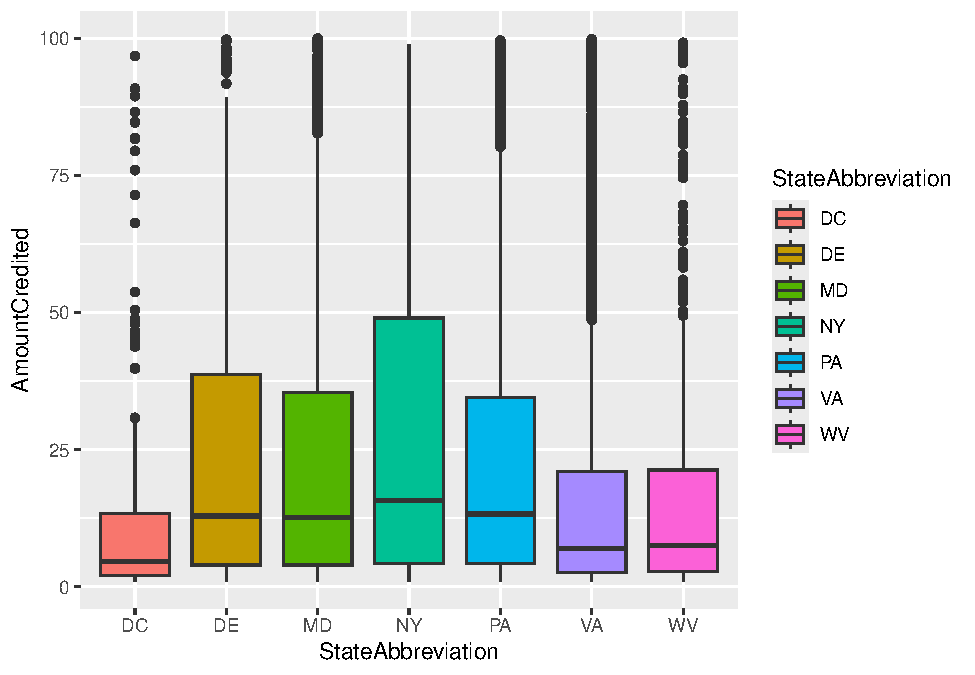
\includegraphics{lab02_files/figure-latex/review3-2.pdf}

\begin{Shaded}
\begin{Highlighting}[]
\CommentTok{\# We can also plot multiple dimensions in our plot using the \textasciigrave{}facet\textasciigrave{} family of commands in ggplot}

\NormalTok{bmps }\SpecialCharTok{\%\textgreater{}\%} 
\NormalTok{  dplyr}\SpecialCharTok{::}\FunctionTok{filter}\NormalTok{(., AmountCredited }\SpecialCharTok{\textgreater{}} \DecValTok{1} \SpecialCharTok{\&}\NormalTok{ AmountCredited }\SpecialCharTok{\textless{}} \DecValTok{100}\NormalTok{) }\SpecialCharTok{\%\textgreater{}\%} 
  \FunctionTok{ggplot}\NormalTok{(., }\FunctionTok{aes}\NormalTok{(}\AttributeTok{x =}\NormalTok{ StateAbbreviation, }\AttributeTok{y =}\NormalTok{ AmountCredited)) }\SpecialCharTok{+}
  \FunctionTok{geom\_boxplot}\NormalTok{(}\FunctionTok{aes}\NormalTok{(}\AttributeTok{fill =}\NormalTok{ StateAbbreviation)) }\SpecialCharTok{+}
  \FunctionTok{facet\_grid}\NormalTok{(Sector}\SpecialCharTok{\textasciitilde{}}\NormalTok{.)}
\end{Highlighting}
\end{Shaded}

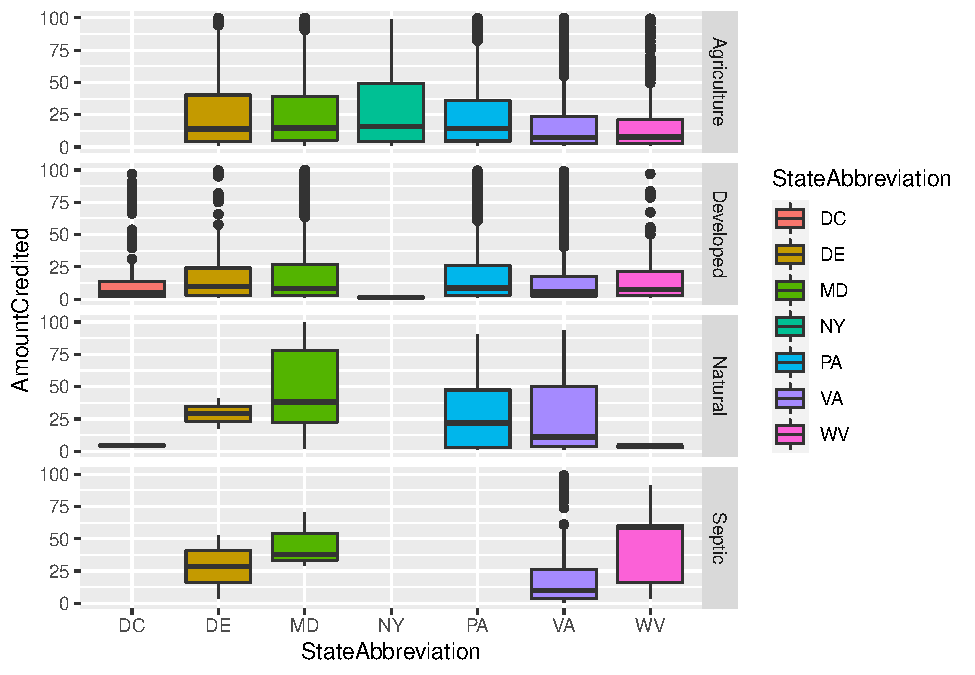
\includegraphics{lab02_files/figure-latex/review3-3.pdf}

The last new item uses the \texttt{\%in\%} command. It's a way to
quickly figure out which elements are inside of another. In that sense,
it's similar to a spatial intersection, but for other types of data.

\begin{Shaded}
\begin{Highlighting}[]
\NormalTok{x }\OtherTok{\textless{}{-}} \FunctionTok{c}\NormalTok{(}\DecValTok{1}\NormalTok{, }\DecValTok{2}\NormalTok{, }\DecValTok{3}\NormalTok{, }\DecValTok{4}\NormalTok{, }\DecValTok{5}\NormalTok{)}

\CommentTok{\# is 7 in our vector?}
\DecValTok{7} \SpecialCharTok{\%in\%}\NormalTok{ x }\CommentTok{\# should be False}
\end{Highlighting}
\end{Shaded}

\begin{verbatim}
## [1] FALSE
\end{verbatim}

\begin{Shaded}
\begin{Highlighting}[]
\DecValTok{2} \SpecialCharTok{\%in\%}\NormalTok{ x }\CommentTok{\# should be True}
\end{Highlighting}
\end{Shaded}

\begin{verbatim}
## [1] TRUE
\end{verbatim}

\begin{Shaded}
\begin{Highlighting}[]
\CommentTok{\# can also do it with vectors}
\FunctionTok{c}\NormalTok{(}\DecValTok{4}\NormalTok{, }\DecValTok{99}\NormalTok{, }\DecValTok{1}\NormalTok{) }\SpecialCharTok{\%in\%}\NormalTok{ x}
\end{Highlighting}
\end{Shaded}

\begin{verbatim}
## [1]  TRUE FALSE  TRUE
\end{verbatim}

Lastly, let's recall using tmap on our data. Also remember you can use
\texttt{sf::st\_make\_valid} to fix offending geometry

\begin{Shaded}
\begin{Highlighting}[]
\NormalTok{counties }\OtherTok{\textless{}{-}}\NormalTok{ sf}\SpecialCharTok{::}\FunctionTok{read\_sf}\NormalTok{(}\StringTok{"../data/CBW/County\_Boundaries.shp"}\NormalTok{)}
\NormalTok{counties }\SpecialCharTok{\%\textgreater{}\%}\NormalTok{ sf}\SpecialCharTok{::}\FunctionTok{st\_is\_valid}\NormalTok{()}
\end{Highlighting}
\end{Shaded}

\begin{verbatim}
##   [1]  TRUE  TRUE  TRUE  TRUE  TRUE  TRUE  TRUE  TRUE  TRUE  TRUE  TRUE  TRUE
##  [13]  TRUE  TRUE  TRUE  TRUE  TRUE  TRUE  TRUE  TRUE  TRUE  TRUE  TRUE  TRUE
##  [25]  TRUE  TRUE  TRUE  TRUE  TRUE  TRUE  TRUE  TRUE  TRUE  TRUE  TRUE  TRUE
##  [37]  TRUE  TRUE  TRUE  TRUE  TRUE  TRUE  TRUE  TRUE  TRUE  TRUE  TRUE  TRUE
##  [49]  TRUE  TRUE  TRUE  TRUE  TRUE  TRUE  TRUE  TRUE  TRUE  TRUE  TRUE  TRUE
##  [61]  TRUE  TRUE  TRUE  TRUE  TRUE  TRUE  TRUE  TRUE  TRUE  TRUE  TRUE  TRUE
##  [73]  TRUE  TRUE  TRUE  TRUE  TRUE  TRUE  TRUE  TRUE  TRUE  TRUE  TRUE  TRUE
##  [85]  TRUE  TRUE  TRUE  TRUE  TRUE  TRUE  TRUE  TRUE  TRUE  TRUE  TRUE  TRUE
##  [97]  TRUE  TRUE  TRUE  TRUE  TRUE  TRUE  TRUE  TRUE  TRUE  TRUE  TRUE  TRUE
## [109]  TRUE  TRUE  TRUE  TRUE  TRUE  TRUE  TRUE  TRUE  TRUE  TRUE  TRUE  TRUE
## [121]  TRUE  TRUE  TRUE  TRUE  TRUE  TRUE  TRUE  TRUE  TRUE  TRUE  TRUE  TRUE
## [133]  TRUE  TRUE  TRUE  TRUE  TRUE  TRUE  TRUE  TRUE  TRUE  TRUE  TRUE  TRUE
## [145]  TRUE  TRUE  TRUE  TRUE  TRUE  TRUE  TRUE  TRUE  TRUE  TRUE  TRUE  TRUE
## [157]  TRUE  TRUE  TRUE  TRUE  TRUE  TRUE  TRUE  TRUE  TRUE  TRUE  TRUE  TRUE
## [169]  TRUE  TRUE  TRUE  TRUE  TRUE  TRUE  TRUE  TRUE  TRUE  TRUE  TRUE  TRUE
## [181]  TRUE  TRUE  TRUE  TRUE  TRUE  TRUE  TRUE  TRUE  TRUE  TRUE  TRUE  TRUE
## [193]  TRUE  TRUE  TRUE  TRUE  TRUE  TRUE  TRUE  TRUE  TRUE  TRUE  TRUE  TRUE
## [205]  TRUE FALSE  TRUE
\end{verbatim}

\begin{Shaded}
\begin{Highlighting}[]
\NormalTok{counties }\OtherTok{\textless{}{-}}\NormalTok{ counties }\SpecialCharTok{\%\textgreater{}\%}\NormalTok{ sf}\SpecialCharTok{::}\FunctionTok{st\_make\_valid}\NormalTok{()}

\CommentTok{\# quick map of the data}
\FunctionTok{tm\_shape}\NormalTok{(counties) }\SpecialCharTok{+} \FunctionTok{tm\_polygons}\NormalTok{(}\AttributeTok{col =} \StringTok{"ALAND10"}\NormalTok{)}
\end{Highlighting}
\end{Shaded}

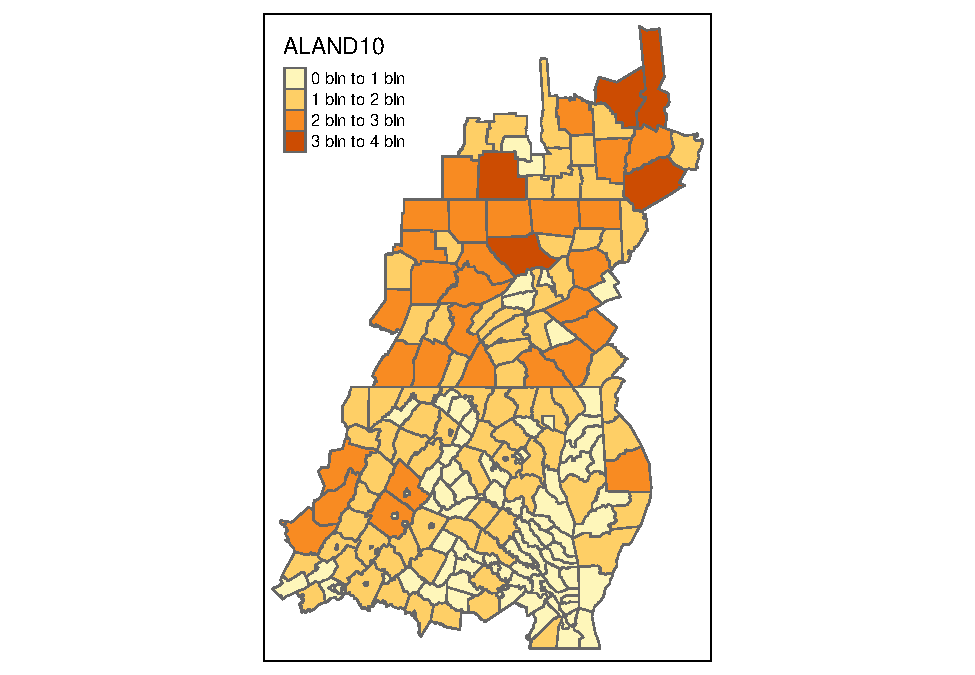
\includegraphics{lab02_files/figure-latex/remembering tmap-1.pdf}

\newpage

\hypertarget{your-tasks}{%
\subsection{Your tasks}\label{your-tasks}}

Using the following data\ldots{}

\begin{Shaded}
\begin{Highlighting}[]
\CommentTok{\# spatial}
\NormalTok{counties }\OtherTok{\textless{}{-}}\NormalTok{ sf}\SpecialCharTok{::}\FunctionTok{read\_sf}\NormalTok{(}\StringTok{"../data/CBW/County\_Boundaries.shp"}\NormalTok{) }\SpecialCharTok{\%\textgreater{}\%}\NormalTok{ sf}\SpecialCharTok{::}\FunctionTok{st\_make\_valid}\NormalTok{()}
\NormalTok{dams }\OtherTok{\textless{}{-}}\NormalTok{ sf}\SpecialCharTok{::}\FunctionTok{read\_sf}\NormalTok{(}\StringTok{"../data/CBW/Dam\_or\_Other\_Blockage\_Removed\_2012\_2017.shp"}\NormalTok{) }\SpecialCharTok{\%\textgreater{}\%}\NormalTok{ sf}\SpecialCharTok{::}\FunctionTok{st\_make\_valid}\NormalTok{()}
\NormalTok{streams }\OtherTok{\textless{}{-}}\NormalTok{ sf}\SpecialCharTok{::}\FunctionTok{read\_sf}\NormalTok{(}\StringTok{"../data/CBW/Streams\_Opened\_by\_Dam\_Removal\_2012\_2017.shp"}\NormalTok{) }\SpecialCharTok{\%\textgreater{}\%}\NormalTok{ sf}\SpecialCharTok{::}\FunctionTok{st\_make\_valid}\NormalTok{()}

\CommentTok{\# aspatial}
\NormalTok{bmps }\OtherTok{\textless{}{-}} \FunctionTok{read\_csv}\NormalTok{(}\StringTok{"../data/CBW/BMPreport2016\_landbmps.csv"}\NormalTok{)}
\end{Highlighting}
\end{Shaded}

\begin{verbatim}
## 
## -- Column specification --------------------------------------------------------
## cols(
##   StateAbbreviation = col_character(),
##   GeographyName = col_character(),
##   Geography = col_character(),
##   Agency = col_character(),
##   BMPShortName = col_character(),
##   BMP = col_character(),
##   BMPType = col_character(),
##   Unit = col_character(),
##   Sector = col_character(),
##   FromLoadSource = col_character(),
##   ToLoadSource = col_character(),
##   AmountSubmitted = col_double(),
##   AmountBackedOut = col_double(),
##   AmountNotBackedOut = col_double(),
##   AmountCredited = col_double(),
##   Excess = col_double(),
##   TotalAmountCredited = col_double(),
##   Cost = col_double()
## )
\end{verbatim}

\ldots complete the following tasks.

Complete each task COMPLETELY USING R CODE. YOU MUST SHOW YOUR WORK FOR
EACH ANSWER. Label your variables sensibly and use comments such that I
can find your answers and your work. The following tasks draw upon
lecture, your assigned readings, and the examples shown above. As
always, there are multiple ways of completing each task. Remember, it's
always a good idea to peform some exploratory data analysis on your own
prior to starting work.

\hypertarget{task-1-aspatial-operations}{%
\subsubsection{Task 1: Aspatial
operations}\label{task-1-aspatial-operations}}

1.1 Calculate summary statistics for the Cost of BMPs for each State
(including DC)

1.2 Make a scatterplot of Cost vs.~TotalAmountCredited, ONLY FOR Units
of type ``Acres''. You may need to apply a data transformation to one or
more axes if the data are heavily skewed.

1.3 Make a boxplot with ``StateAbbreviation'' on the x-axis and
``TotalAmountCredited'' on the y-axis. HOWEVER, the only data I want
plotted are for cover crop BMPs. Note, there are many types of cover
crops in this dataset, and I want you to include them ALL. There are
handy functions within the \texttt{stringr} package that can help you
here.

1.4 make a scatterplot of the dam dataset, this time with ``YEAR'' on
the x-axis and ``STATE'' on y-axis (think of it like a timeline). Assume
no dams were built in year 0, so you'll need to remove those data
points.

1.5 make one last (aspatial) visualization. But this time, it's your
choice what data and plots to use. The only requirement is that you link
two of the datasets together in some manner. Be creative. Make it look
nice (e.g., use proper labels, interesting colors/shading/size).

\hypertarget{task-2-spatial-operations}{%
\subsubsection{Task 2: Spatial
operations}\label{task-2-spatial-operations}}

2.1 Find the 5 longest streams in the `streams opened by dam removal'
dataset

2.2 Find the three counties with the greatest TOTAL length of streams
(opened by dam removal) in them

2.3 Make a map of the counties, shading each county by the total cost of
BMPs funded/implemented in that county. This will required you to join
multiple datasets together

2.4 For each removed dam, find the closest stream segment

2.5 Calculate how many removed dams are (or were) in each state


\end{document}